\documentclass[UTF-8, 12pt]{ctexart}
\usepackage{graphicx}
\setmainfont{Ubuntu}
\setCJKmainfont{WenQuanYi Micro Hei}
\usepackage{fancyhdr}
\title{第一周实验报告}
\author{沈家成}
\date{\today}
\pagestyle{fancy}
\lhead{第一周}
\chead{}
\rhead{\today}
\lfoot{}
\cfoot{\thepage}
\rfoot{}
\renewcommand{\headrulewidth}{0.4pt}
\renewcommand{\headwidth}{\textwidth}
\renewcommand{\footrulewidth}{0pt}

\begin{document}
\maketitle

\section{max1 和 max2 比较}
    \subsection{效率比较}
    \paragraph{}
    max1 调用了两个循环,而第一个循环做了大量无用工作——将 size - 1 个不需要返回的值乘以了 d ,浪费了计算资源。而 max2 只在最后返回值的时候做了乘法,效率较高。
    \begin{figure}[h]
    \centering
    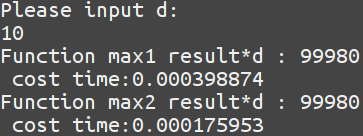
\includegraphics[width = .8\textwidth]{1.png}
    \caption{测试图}
    \end{figure}
    \paragraph{}
    经过测试,比较有 10000 个元素的数组,max1 用的时间是 max2 的 2 倍,差距较大。

    \subsection{安全比较}
    \paragraph{}
    max1 和 max2 都是通过数组传递数据,但是在 max1 中,直接改变了数组中的值,如果之后还需要调用这个数组,就会发现不再是原来的那个数组了。所以,我分别创建了两个测试数组给 max1 和 max2 传递数据,防止这个影响。而 max2 中并没有对数组的赋值,因而更加安全。

    \subsection{小结}
    \paragraph{}
    max1 无论是在效率,还是在数据安全性上都弱于 max2 ,这样的算法改进一举两得,我们应避免 max1 的算法。

\section{最大连续子数列}
    \subsection{效率比较}
    \paragraph{}
    三个算法分别是$O(N^3), O(N^2), O(N)$的时间复杂度。通过挖掘信息,第二个算法剔除了重复的计算,第三个算法剔除了大量不可能的情况,从而降低了时间复杂度。
    \begin{figure}[h]
    \centering
    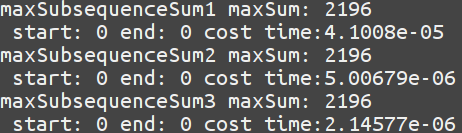
\includegraphics[width = .8\textwidth]{2.png}
    \caption{测试图}
    \end{figure}
    \paragraph{}
    测试中,比较有 90000 个元素的整数序列,三个算法所用的时间越来越少。

    \subsection{可读性比较}
    \paragraph{}
    第一个算法使用穷举法,容易想象其运行过程;第二个算法删去了重复的计算,在理解第一个算法的基础上也可以理解;而第三个算法,第 8 行
    \[ else \ if(thisSum == a[j]) \ startTmp = j; \]
    即使参考了注释也较难理解,需要认识到这行语句是在$ thisSum < 0$之后,加上第一个非负元素的一次循环里起作用。因为$thisSum$被赋值成 0 ,所以加上非负$a[j]$之后,就会进入$thisSum < 0$的$else$分支,产生$thisSum == a[j]$,从而让新的最大子序列的起点跳到$j$。所以第三个算法的可读性远远不如之前两个算法。

    \subsection{小结}
    \paragraph{}
    降低算法的时间复杂度往往也会牺牲代码的可读性。在实际应用中应同时考虑两方面因素,注释中要详细解释难以理解的地方,方便将来的维护。

\section{程序设计题1}
    \subsection{问题分析}
    \paragraph{}
    要判断一个数是不是素数,就是要找因数。1 肯定是因数,因此不用判断。2 有很大的可能是因数,因此应该首先判断。然后就要一个个数字试下去,到了$\frac{N}{2}$时,因为因数肯定小于等于原数的一半,所以就可以停止了。

    \subsection{时间复杂度}
    \paragraph{}
    这个程序调用了一次循环,在最坏的情况下,也就是该数为素数的情况下,会从 2 遍历到$\frac{N}{2}$,共$\frac{N}{2} -1$次循环,即为$O(N)$的时间复杂度。

    \subsection{特殊情况}
    \paragraph{}
    $N$为 1 时,十分特殊,因此直接加了一个判断,如果是 1 就$return \ false;$。因为在循环外面,所以对时间复杂度没有影响。
    \paragraph{}
    $N$为 2 时,2 虽然能被 2 整除,但它是素数。此时,刚好没有进入循环,直接$return \ false;$,是正确的。

    \subsection{小结}
    \paragraph{}
    测试程序时要全面考虑,尤其是特殊情况。在保证正确的情况下,尽量精简代码,提高效率。

\section{程序设计题2}
    \subsection{问题分析}
    \paragraph{}
    这是一个数列求和的问题,如果累加计算的话,就是$O(N)$的时间复杂度,但是要求$O(1)$的时间复杂度,因此不能使用任何循环。为了不使用循环,就需要用数学的方式求出公式。

    \subsection{实现}
    \paragraph{}
    通过观察,可以分为奇偶两种情况。$N$为偶数时,元素两两结合,共有$\frac{N}{2}$个 -1 ,数列和为$\-frac{N}{2}$;$N$为奇数时,先去掉第一个元素 1 ,再两两结合,共有$\frac{N-1}{2}$个 1 ,加上去掉的一个 1 ,数列和为$\frac{N+1}{2}$。这样用一个 if 判断再进行一次计算就可以返回结果了,时间复杂度为$O(1)$。
    
    \subsection{小结}
    \paragraph{}
    通过数学事先求解,可以极大地降低时间复杂度,但是需要一定的数学功底,而且能用数学解决的问题还是小部分。从日常的可行性出发,还是应该更多地从算法的角度,用程序的方法降低时间复杂度。
\end{document}
